\chapter{Specifikacija programske potpore}
		
	\section{Funkcionalni zahtjevi}
			
			\noindent \textbf{Dionici:}
			
			\begin{packed_enum}
				
				\item Organizator konferencije (naručitelj)
				\item Pokrovitelji konferencije
				\item Autori radova
				\item Glasači
				\item Administrator
				\item Natkorisnik
				\item Razvojni tim
				
			\end{packed_enum}
			
			\noindent \textbf{Aktori i njihovi funkcionalni zahtjevi:}
			
			\begin{packed_enum}
				\item  \underbar{Neregistrirani korisnik (inicijator) može:}
				
				\begin{packed_enum}
					
					\item prijaviti se pomoću generičkog korisničkog računa
					
				\end{packed_enum}
				
				\item  \underbar{Korisnik posjetitelj (inicijator) može:}
				
				\begin{packed_enum}
					
					\item registrirati se to jest stvoriti novi korisnički račun za koji su mu potrebni: ime, prezime, lozinka i adresa e-pošte
					\item prijaviti se
					\item pregledavati postere, pri čemu ne može glasati
					
				\end{packed_enum}
			
				\item  \underbar{Registrirani/Prijavljeni korisnik (inicijator) može:}
				
				\begin{packed_enum}
					
					\item pregledavati i glasati za postere pri čemu svaki posjetitelj može glasati najviše za jedan poster
					\item pregledavati promotivne materijale pokrovitelja
					\item gledati video-prijenos
					\item pregledavati i preuzimati fotografije
					\item vidjeti informacije o mjestu održavanja koje uključuju vremenske uvjete, vremensku prognozu i kartu
					\item \textcolor{red}{pristupiti rezultatima jednom kad postanu dostupni}
					\item odjaviti se
				
				\end{packed_enum}
				
				\item  \underbar{Korisnik (inicijator):}
				
				\begin{packed_enum}
					
					\item generalizacija korisnika posjetitelja i registriranog korisnika
					
				\end{packed_enum}
				
				\item \underbar{Administrator (inicijator) može:}
				
				\begin{packed_enum}
					
					\item prijaviti i ukloniti autore, radove i postere
					\item obrisati određene korisničke račune
					\item pristupiti svim podacima vezanim za konferenciju
					\item definirati sve uvjete za rad sustava
					
				\end{packed_enum}
				
				\item \underbar{Natkorisnik (inicijator) može:}
				
				\begin{packed_enum}
				
					\item stvoriti novu konferenciju
					\item dodati administratora za konferenciju
					\item izbrisati konferenciju

				\end{packed_enum}
				
				\item \underbar{Baza podataka (sudionik):}
				
				\begin{packed_enum}
					
					\item pohranjuje podatke o korisnicima
					\item pohranjuje podatke o digitalnim posterima, broju njihovih glasova, njihovim autorima
					\item pohranjuje fotografije uslikane za vrijeme trajanja konferencije
					
				\end{packed_enum}
				
				\item \underbar{Poslužitelj strujanja (sudionik):}
				
				\begin{packed_enum}
					
					\item pruža uslugu video prijenosa konferencije
				
				\end{packed_enum}
				
				\item \underbar{Poslužitelj vremenske prognoze (sudionik):}
				
				\begin{packed_enum}
					
					\item poslužuje potrebne podatke vezane za prognozu vremena
					
				\end{packed_enum}
				
				\item \underbar{Poslužitelj karte (sudionik):}
				
				\begin{packed_enum}
					
					\item poslužuje potrebne podatke za prikaz karte
					
				\end{packed_enum}
				
				\item \underbar{Poslužitelj e-pošte (sudionik):}
				
				\begin{packed_enum}
					
					\item omogućuje aplikaciji da šalje e-poruke korisnicima
					
				\end{packed_enum}
				
			\end{packed_enum}
			
			\eject 
			
			
				
			\subsection{Obrasci uporabe}
					
					\newcounter{UseCaseCounter}
					\setcounter{UseCaseCounter}{1}
					
					\noindent \underbar{\textbf{UC\theUseCaseCounter \stepcounter{UseCaseCounter} - Pristup konferenciji}}
					\begin{packed_item}
						
						\item \textbf{Glavni sudionik: } Neregistrirani korisnik
						\item  \textbf{Cilj:} Pristupiti konferenciji kao korisnik posjetitelj
						\item  \textbf{Sudionici:} Baza podataka
						\item  \textbf{Preduvjet:} Nema preduvjeta
						\item  \textbf{Opis osnovnog tijeka:}
						
						\item[] \begin{packed_enum}
							
							\item Korisnik odabire konferenciju kojoj želi pristupiti
							\item Upisuje generičko korisničko ime (predviđenu adresu e-pošte) i lozinku za odabranu konferenciju
							\item Otvara se pregled konferencije s mogućnostima korisnika posjetitelja
						\end{packed_enum}
						
						\item  \textbf{Opis mogućih odstupanja:}
						
						\item[] \begin{packed_item}
							
							\item[2.a] Pogrešno generičko ime ili lozinka
							\item[] \begin{packed_enum}
								
								\item Sustav obavještava korisnika o upisu pogrešne lozinke ili imena
								\item Povratak na zaslon za pristup konferenciji
								
							\end{packed_enum}
							
						\end{packed_item}
					\end{packed_item}
					
					%UC2
					\noindent \underbar{\textbf{UC\theUseCaseCounter \stepcounter{UseCaseCounter} - Prijava}}
					\begin{packed_item}
						
						\item \textbf{Glavni sudionik: } Registrirani korisnik
						\item  \textbf{Cilj:} Pristup svim korisničkim funkcionalnostima aplikacije
						\item  \textbf{Sudionici:} Baza podataka
						\item  \textbf{Preduvjet:} Nema preduvjeta
						\item  \textbf{Opis osnovnog tijeka:}
						
						\item[] \begin{packed_enum}
							
							\item Otvara se prozor u koji korisnik upisuje podatke
							\item Provjera postoji li korisnik u bazi podataka
							\item Ako korisnik postoji, otvara se prozor s posterima, a korisnik je prijavljen
						\end{packed_enum}
						
						\item  \textbf{Opis mogućih odstupanja:}
						
						\item[] \begin{packed_item}
							
							\item[3.a] Korisnik ne postoji u bazi podataka
							\item[] \begin{packed_enum}
								
								\item Sustav obavještava korisnika o upisu pogrešne lozinke ili adrese e-pošte
								
							\end{packed_enum}
							
						\end{packed_item}
					\end{packed_item}
					
					%UC3
					\noindent \underbar{\textbf{UC\theUseCaseCounter \stepcounter{UseCaseCounter} - Registracija}}
					\begin{packed_item}
					
						\item \textbf{Glavni sudionik: } Korisnik posjetitelj
						\item  \textbf{Cilj:} Stvoriti vlastiti korisnički račun
						\item  \textbf{Sudionici:} Baza podataka
						\item  \textbf{Preduvjet:} Korisnik je prijavljen s generičkim računom
						\item  \textbf{Opis osnovnog tijeka:}
						
						\item[] \begin{packed_enum}
							
							\item Korisnik odabire opciju za registraciju
							\item Korisnik unosi potrebne korisničke podatke
							\item Korisnik prima obavijest o uspješnoj registraciji

						\end{packed_enum}
						
						\item  \textbf{Opis mogućih odstupanja:}
						
						\item[] \begin{packed_item}
							
							\item[2.a] Odabir već zauzete adrese e-pošte, unos korisničkog podatka u nedozvoljenom formatu ili pružanje neispravne adrese e-pošte
							\item[] \begin{packed_enum}
								
								\item Sustav obavještava korisnika o neuspjelom upisu i vraća ga na stranicu za registraciju
								\item Korisnik mijenja potrebne podatke te završava unos ili odustaje od registracije
								
							\end{packed_enum}
							
						\end{packed_item}
					\end{packed_item}
					
					\noindent \underbar{\textbf{UC\theUseCaseCounter \stepcounter{UseCaseCounter} - Odjava}}
					\begin{packed_item}
						
						\item \textbf{Glavni sudionik: } Registrirani korisnik
						\item  \textbf{Cilj:} Odjaviti se iz konferencije
						\item  \textbf{Sudionici:} Baza podataka
						\item  \textbf{Preduvjet:} Nema preduvjeta
						\item  \textbf{Opis osnovnog tijeka:}
						
						\item[] \begin{packed_enum}
							
							\item Korisnik odabire opciju za odjavu
							\item Korisnik potvrđuje odjavu
							\item Povratak na zaslon za pristup konferenciji
						\end{packed_enum}
						
						\item  \textbf{Opis mogućih odstupanja:}
						
						\item[] \begin{packed_item}
							
							\item[2.a] Korisnik odustaje od odjave
							\item[] \begin{packed_enum}
								
								\item Povratak na prethodni zaslon
								
							\end{packed_enum}
							
						\end{packed_item}
					\end{packed_item}
				
					%UC4
					\noindent \underbar{\textbf{UC\theUseCaseCounter \stepcounter{UseCaseCounter} - Pregled galerije postera}}
					\begin{packed_item}
						
						\item \textbf{Glavni sudionik: } Korisnik
						\item  \textbf{Cilj:} Pregled svih postavljenih postera
						\item  \textbf{Sudionici:} Baza podataka
						\item  \textbf{Preduvjet:} Korisnik je prijavljen
						\item  \textbf{Opis osnovnog tijeka:}
						
						\item[] \begin{packed_enum}
							
							\item Otvara se prozor s posterima
							
						\end{packed_enum}
							
					\end{packed_item}
					
					\noindent \underbar{\textbf{UC\theUseCaseCounter \stepcounter{UseCaseCounter} - Pregled promotivnih materijala}}
					\begin{packed_item}

						\item \textbf{Glavni sudionik: } Registrirani korisnik
						\item  \textbf{Cilj:} Pregledati promotivne materijale pokrovitelja konferencije
						\item  \textbf{Sudionici:} Baza podataka
						\item  \textbf{Preduvjet:} Korisnik je registriran i prijavljen
						\item  \textbf{Opis osnovnog tijeka:}
						
						\item[] \begin{packed_enum}
							
							\item Korisnik odabire opciju za promotivne materijale
							\item Otvara se stranica s promotivnim materijalima

						\end{packed_enum}

					\end{packed_item}
					
					\noindent \underbar{\textbf{UC\theUseCaseCounter \stepcounter{UseCaseCounter} - Pregled informacija o konferenciji}}
					\begin{packed_item}
						
						\item \textbf{Glavni sudionik: } Registrirani korisnik
						\item  \textbf{Cilj:} Pregledati informacije o mjestu održavanja konferencije, uključujući kartu i informacije o trenutnim vremenskim uvjetima i vremenskoj prognozi za navedenu lokaciju
						\item  \textbf{Sudionici:} Baza podataka
						\item  \textbf{Preduvjet:} Korisnik je registriran i prijavljen
						\item  \textbf{Opis osnovnog tijeka:}
						
						\item[] \begin{packed_enum}
							
							\item Sve informacije se nalaze na stranici konferencije
						\end{packed_enum}
					\end{packed_item}
					
					\noindent \underbar{\textbf{UC\theUseCaseCounter \stepcounter{UseCaseCounter} - Pregled galerije fotografija}}
					\begin{packed_item}
						
						\item \textbf{Glavni sudionik: } Registriran korisnik
						\item  \textbf{Cilj:} Pregledati galeriju fotografija
						\item  \textbf{Sudionici:} Baza podataka
						\item  \textbf{Preduvjet:} Korisnik je registriran i prijavljen
						\item  \textbf{Opis osnovnog tijeka:}
						
						\item[] \begin{packed_enum}
							
							\item Korisnik odabire opciju za prikaz galerije fotografija
							\item Otvara se galerija fotografija
						\end{packed_enum}
						
						\item  \textbf{Opis mogućih odstupanja:}
						
						\item[] \begin{packed_item}
							\item[2.a] Nema učitanih fotografija
							\item[] \begin{packed_enum}			
								\item Prikazuje se poruka o nedostatku fotografija
							\end{packed_enum}
						\end{packed_item}
					\end{packed_item}
					
					\noindent \underbar{\textbf{UC\theUseCaseCounter \stepcounter{UseCaseCounter} - Pregled fotografije s konferencije}}
					\begin{packed_item}
						
						\item \textbf{Glavni sudionik: } Registrirani korisnik
						\item  \textbf{Cilj:} Pregledati izabranu fotografiju iz galerije fotografija
						\item  \textbf{Sudionici:} Baza podataka
						\item  \textbf{Preduvjet:} Posjetitelj je prijavljen te je otvorena galerija fotografija
						\item  \textbf{Opis osnovnog tijeka:}
						
						\item[] \begin{packed_enum}
							
							\item Korisnik odabire fotografiju iz galerije
							\item Odabrana fotografije prikaže se uvećana
							\item Korisnik izlazi iz pregleda fotografije
							
						\end{packed_enum}
						
						\item  \textbf{Opis mogućih odstupanja:}
						
						\item[] \begin{packed_item}
							
							\item[1.a] Nema fotografija u galeriji
							\item[] \begin{packed_enum}
								
								\item Klik na prazno područje galerije ne čini ništa
								
							\end{packed_enum}
							
						\end{packed_item}
					\end{packed_item}
					
					\noindent \underbar{\textbf{UC\theUseCaseCounter \stepcounter{UseCaseCounter} - Preuzimanje fotografija s konferencije}}
					\begin{packed_item}
						
						\item \textbf{Glavni sudionik: } Registrirani korisnik
						\item  \textbf{Cilj:} Preuzeti izabranu fotografiju iz galerije
						\item  \textbf{Sudionici:} Baza podataka
						\item  \textbf{Preduvjet:} Posjetitelj je prijavljen, otvorena je galerija fotografija, galerija nije prazna
						\item  \textbf{Opis osnovnog tijeka:}
						
						\item[] \begin{packed_enum}
							
							\item Korisnik odabire opciju za preuzimanje fotografije
							\item Odabrane fotografije se preuzimaju na uređaj
							
						\end{packed_enum}
						
					\end{packed_item}
					
					\noindent \underbar{\textbf{UC\theUseCaseCounter \stepcounter{UseCaseCounter} - Prikaz video prijenosa}}
					\begin{packed_item}
						
						\item \textbf{Glavni sudionik: } Registrirani korisnik
						\item  \textbf{Cilj:} Gledati video prijenos konferencije
						\item  \textbf{Sudionici:} Poslužitelj strujanja
						\item  \textbf{Preduvjet:} Korisnik je registriran i prijavljen
						\item  \textbf{Opis osnovnog tijeka:}
						
						\item[] \begin{packed_enum}
							
							\item Korisnik odabire opciju za pokretanje video prijenosa
							
						\end{packed_enum}
						
						\item  \textbf{Opis mogućih odstupanja:}
						
						\item[] \begin{packed_item}
							
							\item[2.a] Tehnički problemi u prijenosu konferencije na poslužitelj strujanja
							\item[] \begin{packed_enum}
								
								\item Poslužitelj strujanja obavještava korisnika da video prijenos trenutno nije dostupan
								
							\end{packed_enum}
							
						\end{packed_item}
					\end{packed_item}
					
					\noindent \underbar{\textbf{UC\theUseCaseCounter \stepcounter{UseCaseCounter} - Pregled digitalnog postera ili prezentacije}}
					\begin{packed_item}
						
						\item \textbf{Glavni sudionik: } Korisnik
						\item  \textbf{Cilj:} Pregledati poster
						\item  \textbf{Sudionici:} Baza podataka
						\item  \textbf{Preduvjet:} Pregled galerije postera
						\item  \textbf{Opis osnovnog tijeka:}
						
						\item[] \begin{packed_enum}
							
							\item Korisnik je odabrao digitalni poster
							\item Korisnik pregledava informacije o digitalnom posteru
							\item Korisnik izlazi iz pregleda digitalnog postera
						\end{packed_enum}
						
					\end{packed_item}
					
					\noindent \underbar{\textbf{UC\theUseCaseCounter \stepcounter{UseCaseCounter} - Glasovanje}}
					\begin{packed_item}
						
						\item \textbf{Glavni sudionik: } Registrirani korisnik
						\item  \textbf{Cilj:} Glasovati za rad
						\item  \textbf{Sudionici:} Baza podataka
						\item  \textbf{Preduvjet:} Prijava, Pregled digitalnog postera
						\item  \textbf{Opis osnovnog tijeka:}
						
						\item[] \begin{packed_enum}
							
							\item Korisnik odabire opciju glasovanja
							\item U sustavu se evidentira korisnikovo glasovanje
						\end{packed_enum}
						
						\item  \textbf{Opis mogućih odstupanja:}
						
						\item[] \begin{packed_item}
							
							\item[2.a] Korisnik je već glasovao
							\item[] \begin{packed_enum}
								\item Korisnik je obaviješten o nemogućnosti daljnjeg glasovanja
							\end{packed_enum}
						\end{packed_item}
					\end{packed_item}
					
					\noindent \underbar{\textbf{UC\theUseCaseCounter \stepcounter{UseCaseCounter} - Pregled rezultata glasovanja}}
					\begin{packed_item}
						
						\item \textbf{Glavni sudionik: } Registrirani korisnik
						\item  \textbf{Cilj:} Uvid u rezultate glasovanja
						\item  \textbf{Sudionici:} Baza podataka
						\item  \textbf{Preduvjet:} Prijava, registrirani korisnik
						\item  \textbf{Opis osnovnog tijeka:}
						
						\item[] \begin{packed_enum}
							
							\item Korisnik odabire opciju rezultati glasovanja u izborniku
							\item Otvara se zasebna stranica gdje je rang lista autora/radova
							\item Korisnik pregledava rang listu
						\end{packed_enum}
						
					\end{packed_item}
					
					\noindent \underbar{\textbf{UC\theUseCaseCounter \stepcounter{UseCaseCounter} - Brisanje korisničkog računa}}
					\begin{packed_item}
						
						\item \textbf{Glavni sudionik: }Administrator
						\item  \textbf{Cilj:} Izbrisati korisnički račun
						\item  \textbf{Sudionici:} Baza podataka
						\item  \textbf{Preduvjet:} Administrator je prijavljen
						\item  \textbf{Opis osnovnog tijeka:}
						
						\item[] \begin{packed_enum}
							
							\item Administrator otvori popis registriranih korisnika
							\item Administrator odabire korisnički račun
							\item Administrator odlučuje obrisati korisnički račun
							\item Administratora se traži da potvrdi brisanje korisničkog računa
							\item Otvara se popis registriranih korisnika
						\end{packed_enum}
						
						\item  \textbf{Opis mogućih odstupanja:}
						
						\item[] \begin{packed_item}
							
							\item[4.a] Administrator odlučuje ne obrisati korisnički račun
							\item[] \begin{packed_enum}			
								\item Povratak na popis korisničkih računa
							\end{packed_enum}
						\end{packed_item}
					\end{packed_item}
					
					\noindent \underbar{\textbf{UC\theUseCaseCounter \stepcounter{UseCaseCounter} - Upravljanje digitalnim posterima}}
					\begin{packed_item}
						
						\item \textbf{Glavni sudionik: } Administrator
						\item  \textbf{Cilj:} Dodavanje ili brisanje postavljenih postera s početne stranice
						\item  \textbf{Sudionici:} Baza podataka
						\item  \textbf{Preduvjet:} Prijavljen je administrator, otvorena stranica s posterima
						\item  \textbf{Opis osnovnog tijeka:}
						
						\item[] \begin{packed_enum}
							
							\item Administrator pritiskom na gumb otvara posebno sučelje za upravljanje posterima
						\end{packed_enum}
						
						
					\end{packed_item}
					
					\noindent \underbar{\textbf{UC\theUseCaseCounter \stepcounter{UseCaseCounter} - Dodavanje digitalnog postera}}
					\begin{packed_item}
						
						\item \textbf{Glavni sudionik: } Administrator
						\item  \textbf{Cilj:} Dodavanje novog postera
						\item  \textbf{Sudionici:} Baza Podataka
						\item  \textbf{Preduvjet:} Administrator je prijavljen, otvoreno je sučelje za upravljanje posterima
						\item  \textbf{Opis osnovnog tijeka:}
						
						\item[] \begin{packed_enum}
							
							\item Administrator pritišće gumb za dodavanje novog postera
							\item Otvara se prozor s mogućnošću odabira lokalne datoteke i unosa podataka o posteru
							\item Administrator odabire željenu datoteku za prijenos u bazu podataka aplikacije
							\item Administrator potvrđuje promjene
						\end{packed_enum}
						
						\item  \textbf{Opis mogućih odstupanja:}
						
						\item[] \begin{packed_item}
							
							\item[2.a] Administrator odustaje od dodavanja postera
							\item[] \begin{packed_enum}
								
								\item Povratak na sučelje za upravljanje posterima
							\end{packed_enum}
							
						\end{packed_item}
					\end{packed_item}
					
					\noindent \underbar{\textbf{UC\theUseCaseCounter \stepcounter{UseCaseCounter} - Brisanje digitalnog postera}}
					\begin{packed_item}
						
						\item \textbf{Glavni sudionik: } Administrator
						\item  \textbf{Cilj:} Brisanje odabranog digitalnog postera
						\item  \textbf{Sudionici:} Baza podataka
						\item  \textbf{Preduvjet:} Otvoreno sučelje za upravljanje digitalnih postera, prijavljen je administrator
						\item  \textbf{Opis osnovnog tijeka:}
						
						\item[] \begin{packed_enum}
							
							\item Administrator odabire digitalni poster
							\item Administrator odabire opciju za brisanje digitalnog postera
							\item Pojavljuje se upit za potvrdu brisanja
							\item Ako je upit potvrđen poster se briše iz baze podataka, u protivnom se vraća na sučelje za upravljanje posterima
						\end{packed_enum}
						
						\item  \textbf{Opis mogućih odstupanja:}
						
						\item[] \begin{packed_item}
							
							\item[4.a] Administrator odustaje od brisanja
							\item[] \begin{packed_enum}
								
								\item Povratak na sučelje za upravljanje posterima
							\end{packed_enum}
							
						\end{packed_item}
					\end{packed_item}
					
					\noindent \underbar{\textbf{UC\theUseCaseCounter \stepcounter{UseCaseCounter} - Upravljanje fotografijama}}
					\begin{packed_item}
						
						\item \textbf{Glavni sudionik: }Administrator
						\item  \textbf{Cilj:} Otvaranje sučelja za uređivanje fotografija
						\item  \textbf{Sudionici:} Baza podataka
						\item  \textbf{Preduvjet:} Prijavljen je administrator
						\item  \textbf{Opis osnovnog tijeka:}
						
						\item[] \begin{packed_enum}
							
							\item Administrator odabire opciju za upravljanje fotografijama
							\item Otvara se sučelje za upravljanje fotografijama
						\end{packed_enum}
						
					\end{packed_item}
					
					\noindent \underbar{\textbf{UC\theUseCaseCounter \stepcounter{UseCaseCounter} - Dodavanje fotografije}}
					\begin{packed_item}
						
						\item \textbf{Glavni sudionik: }Administrator
						\item  \textbf{Cilj:} Dodavanje nove fotografije u galeriju fotografija
						\item  \textbf{Sudionici:} Baza podataka
						\item  \textbf{Preduvjet:} Prijavljen je administrator, otvoreno je sučelje za upravljanje fotografijama
						\item  \textbf{Opis osnovnog tijeka:}
						
						\item[] \begin{packed_enum}
							
							\item Administrator odabire opciju za dodavanje nove fotografije
							\item Administrator odabire jednu ili više fotografija s vlastitog računala
							\item Administrator potvrđuje promjene
							\item Povratak na sučelje za upravljanje fotografijama
						\end{packed_enum}
						
						\item  \textbf{Opis mogućih odstupanja:}
						
						\item[] \begin{packed_item}
							
							\item[2.a] Administrator je odabrao datoteku koja nije podržanog tipa
							\item[] \begin{packed_enum}
								
								\item Sustav obavještava administratora o odabiru datoteke nepodržanog tipa
								\item Odbacivanje promjena
								\item Povratak na sučelje za upravljanje fotografijama
								
							\end{packed_enum}
							
							\item[3.a] Administrator odustaje od dodavanja fotografije
							\item[] \begin{packed_enum}
								
								\item Povratak na sučelje za upravljanje fotografijama
							
							\end{packed_enum}
							
						\end{packed_item}
					\end{packed_item}
					
					\noindent \underbar{\textbf{UC\theUseCaseCounter \stepcounter{UseCaseCounter} - Brisanje fotografije}}
					\begin{packed_item}
						
						\item \textbf{Glavni sudionik: }Administrator
						\item  \textbf{Cilj:} Brisanje odabrane fotografije
						\item  \textbf{Sudionici:} Baza podataka
						\item  \textbf{Preduvjet:} Prijavljen je administrator, otvoreno sučelje za upravljanje fotografijama
						\item  \textbf{Opis osnovnog tijeka:}
						
						\item[] \begin{packed_enum}
							
							\item Administrator odabire fotografiju
							\item Administrator odabire opciju za brisanje fotografije
							\item Potvrda brisanja odabrane fotografije iz baze podataka
							\item Povratak na sučelje za upravljanje fotografijama
						\end{packed_enum}
						
						\item  \textbf{Opis mogućih odstupanja:}
						
						\item[] \begin{packed_item}
							
							\item[4.a] Administrator odustaje od brisanja fotografije
							\item[] \begin{packed_enum}
								
								\item Povratak na sučelje za upravljanje fotografijama
								
							\end{packed_enum}
							
						\end{packed_item}
					\end{packed_item}
					
					\noindent \underbar{\textbf{UC\theUseCaseCounter \stepcounter{UseCaseCounter} - Upravljanje promotivnim materijalima}}
					\begin{packed_item}
						
						\item \textbf{Glavni sudionik: }Administrator
						\item  \textbf{Cilj:} Otvaranje sučelja za upravljanje promotivnim materijalima
						\item  \textbf{Sudionici:} Baza podataka
						\item  \textbf{Preduvjet:} Prijavljen je administrator
						\item  \textbf{Opis osnovnog tijeka:}
						
						\item[] \begin{packed_enum}
							
							\item Administrator odabire opciju za otvaranje sučelja za upravljanje promotivnim materijalima
							\item Otvara se sučelje za upravljanje promotivnim materijalima
						\end{packed_enum}
						
					\end{packed_item}
					
					\noindent \underbar{\textbf{UC\theUseCaseCounter \stepcounter{UseCaseCounter} - Dodavanje promotivnih materijala}}
					\begin{packed_item}
						
						\item \textbf{Glavni sudionik: }Administrator
						\item  \textbf{Cilj:} Dodati nove promotivne materijale
						\item  \textbf{Sudionici:} Baza podataka
						\item  \textbf{Preduvjet:} Prijavljen je administrator, otvoreno je sučelje za upravljanje promotivnim materijalima
						\item  \textbf{Opis osnovnog tijeka:}
						
						\item[] \begin{packed_enum}
							
							\item Administrator odabire opciju za dodavanje novog promotivnog materijala
							\item Administrator unosi potrebne podatke
							\item Administrator potvrđuje promjene
							\item Povratak na sučelje za upravljanje promotivnim materijalima
						\end{packed_enum}
						
						\item  \textbf{Opis mogućih odstupanja:}
						
						\item[] \begin{packed_item}
							
							\item[4.a] Administrator odustaje od dodavanja promotivnih materijala
							\item[] \begin{packed_enum}
								
								\item Povratak na sučelje za upravljanje promotivnim materijalima
								
							\end{packed_enum}
							
						\end{packed_item}
					\end{packed_item}
					
					\noindent \underbar{\textbf{UC\theUseCaseCounter \stepcounter{UseCaseCounter} - Brisanje promotivnih materijala}}
					\begin{packed_item}
						
						\item \textbf{Glavni sudionik: }Administrator
						\item  \textbf{Cilj:} Brisanje odabranih promotivnih materijala
						\item  \textbf{Sudionici:} Baza podataka
						\item  \textbf{Preduvjet:} Prijavljen je administrator, otvoreno sučelje za upravljanje promotivnim materijalima
						\item  \textbf{Opis osnovnog tijeka:}
						
						\item[] \begin{packed_enum}
							
							\item Administrator odabire opciju za brisanje promotivnog materijala
							\item Potvrda brisanja odabranog promotivnog materijala iz baze podataka
							\item Povratak na sučelje za upravljanje fotografijama
						\end{packed_enum}
						
						\item  \textbf{Opis mogućih odstupanja:}
						
						\item[] \begin{packed_item}
							
							\item[2.a] Administrator odustaje od brisanja materijala
							\item[] \begin{packed_enum}
								
								\item Povratak na sučelje za upravljanje promotivnim materijalima
								
							\end{packed_enum}
							
						\end{packed_item}
					\end{packed_item}
					
					\noindent \underbar{\textbf{UC\theUseCaseCounter \stepcounter{UseCaseCounter} - Upravljanje video prijenosom}}
					\begin{packed_item}
						
						\item \textbf{Glavni sudionik: }Administrator
						\item  \textbf{Cilj:} Promijeniti video prijenos
						\item  \textbf{Sudionici:} Baza podataka
						\item  \textbf{Preduvjet:} Prijavljen je administrator
						\item  \textbf{Opis osnovnog tijeka:}
						
						\item[] \begin{packed_enum}
							
							\item Administrator odabire opciju za upravljanje video prijenosom
							\item Otvara se sučelje za upravljanje video prijenosom
							\item Administrator mijenja URL video prijenosa
							\item Administrator potvrđuje promjene
							\item Izlazak iz sučelja za upravljanje video prijenosom
						\end{packed_enum}
						
						\item  \textbf{Opis mogućih odstupanja:}
						
						\item[] \begin{packed_item}
							
							\item[4.a] Administrator odustaje od promjene video prijenosa
							\item[] \begin{packed_enum}
								
								\item Izlazak iz sučelja za upravljanje video prijenosom
								
							\end{packed_enum}
							
						\end{packed_item}
						
					\end{packed_item}
					
					\noindent \underbar{\textbf{UC\theUseCaseCounter \stepcounter{UseCaseCounter} - Upravljanje podacima o konferenciji}}
					\begin{packed_item}
						
						\item \textbf{Glavni sudionik: }Administrator
						\item  \textbf{Cilj:} Promijeniti trajanje konferencije
						\item  \textbf{Sudionici:} Baza podataka
						\item  \textbf{Preduvjet:} Prijavljen je administrator
						\item  \textbf{Opis osnovnog tijeka:}
						
						\item[] \begin{packed_enum}
							
							\item Administrator odabire opciju za upravljanjem trajanja konferencije
							\item Otvara se sučelje za upravljanjem trajanja konferencije
							\item Administrator odabire vrijeme početka i kraja konferencije
							\item Administrator potvrđuje promjene
							\item Izlazak iz sučelja za upravljanjem trajanja
						\end{packed_enum}
						
						\item  \textbf{Opis mogućih odstupanja:}
						
						\item[] \begin{packed_item}
							
							\item[1.a] Administrator odabire opciju za upravljanjem lokacije konferencije
							\item[] \begin{packed_enum}
								
								\item Otvara se sučelje za upravljanje lokacijom
								\item Administrator odabire lokaciju konferencije
								\item Administrator potvrđuje promjene
								\item Izlazak iz sučelja za upravljanje lokacijom
								
							\end{packed_enum}
							
							\item[4.a] Administrator odustaje od promjene trajanja/lokacije
							\item[] \begin{packed_enum}
								
								\item Izlazak iz sučelja za upravljanjem trajanja/lokacijom
								
							\end{packed_enum}
							
						\end{packed_item}
						
					\end{packed_item}
					
					\noindent \underbar{\textbf{UC\theUseCaseCounter \stepcounter{UseCaseCounter} - Dohvat vremenske prognoze}}
					\begin{packed_item}
						
						\item \textbf{Glavni sudionik: } Poslužitelj vremenske prognoze
						\item  \textbf{Cilj:} Dohvatiti podatke o vremenskoj prognozi
						\item  \textbf{Sudionici:} -
						\item  \textbf{Preduvjet:} Prijavljen je registrirani korisnik, aplikacija je pokrenuta
						\item  \textbf{Opis osnovnog tijeka:}
						
						\item[] \begin{packed_enum}
							
							\item Nakon prijave registriranog korisnika aplikacija šalje zahtjev za podacima poslužitelju vremenske prognoze
						\end{packed_enum}
							
					\end{packed_item}	
					
						\noindent \underbar{\textbf{UC\theUseCaseCounter \stepcounter{UseCaseCounter} - Dohvat karte}}
					\begin{packed_item}
						
						\item \textbf{Glavni sudionik: } Poslužitelj karte
						\item  \textbf{Cilj:} Dohvatiti kartu
						\item  \textbf{Sudionici:} -
						\item  \textbf{Preduvjet:} Prijavljen je registrirani korisnik, aplikacija je pokrenuta
						\item  \textbf{Opis osnovnog tijeka:}
						
						\item[] \begin{packed_enum}
							
							\item Nakon prijave registriranog korisnika aplikacija šalje zahtjev za podacima poslužitelju karte
						\end{packed_enum}
						
					\end{packed_item}	
					
					\noindent \underbar{\textbf{UC\theUseCaseCounter \stepcounter{UseCaseCounter} - Slanje poruke e-pošte}}
					\begin{packed_item}
						
						\item \textbf{Glavni sudionik: } Poslužitelj e-pošte
						\item  \textbf{Cilj:} Poslati poruku e-pošte
						\item  \textbf{Sudionici:} Baza podataka
						\item  \textbf{Preduvjet:} Završen postupak glasovanja
						\item  \textbf{Opis osnovnog tijeka:}
						
						\item[] \begin{packed_enum}
							
							\item Traženje i dohvat adresa e-pošte autora prvih triju radova po broju glasova iz baze podataka
							\item Slanje poziva na dodjelu nagrade autorima nagrađenih radova e-porukom i notifikacijom na aplikaciji
							\item Slanje obavijesti o mjestu i vremenu dodjele nagrade svim registriranim korisnicima e-porukom i notifikacijom na aplikaciji
							\item Dohvaćanje adresa e-pošte svih autora natjecateljskih radova
							\item Slanje obavijesti o rangu svim sudionicima natjecanja e-porukom i notifikacijom na aplikaciji
						\end{packed_enum}
						
					\end{packed_item}
					
					\noindent \underbar{\textbf{UC\theUseCaseCounter \stepcounter{UseCaseCounter} - Dodavanje konferencije}}
					\begin{packed_item}
						
						\item \textbf{Glavni sudionik: } Natkorisnik
						\item  \textbf{Cilj:} Stvoriti novu konferenciju
						\item  \textbf{Sudionici:} Baza podataka
						\item  \textbf{Preduvjet:} Prijavljen je natkorisnik
						\item  \textbf{Opis osnovnog tijeka:}
						
						\item[] \begin{packed_enum}
							
							\item Korisnik odabire opciju za stvaranje nove konferencije
							\item Korisnik se prijavljuje podacima za prijavu natkorisnika
							\item Otvara se obrazac za unos naziva i trajanja konferencije i dodavanje administratora konferencije
							\item Natkorisnik potvrđuje promjene
							\item Povratak na zaslon za odabir konferencije
							
						\end{packed_enum}
						
						\item  \textbf{Opis mogućih odstupanja:}
						
						\item[] \begin{packed_item}
							
							\item[4.a] Natkorisnik odustaje od dodavanja konferencije
							\item[] \begin{packed_enum}
								
								\item Povratak na zaslon za odabir konferencije
								
							\end{packed_enum}
							
						\end{packed_item}
						
					\end{packed_item}
					
					\noindent \underbar{\textbf{UC\theUseCaseCounter \stepcounter{UseCaseCounter} - Brisanje konferencije}}
					\begin{packed_item}
						
						\item \textbf{Glavni sudionik: } Natkorisnik
						\item  \textbf{Cilj:} Izbrisati konferenciju
						\item  \textbf{Sudionici:} Baza podataka
						\item  \textbf{Preduvjet:} Prijavljen je natkorisnik
						\item  \textbf{Opis osnovnog tijeka:}
						
						\item[] \begin{packed_enum}
							
							\item Korisnik odabire jednu od konferencija koju želi obrisati
							\item Korisnik se prijavljuje podacima za prijavu natkorisnika
							\item Traži se potvrda brisanja
							\item Natkorisnik potvrđuje promjene
							\item Povratak na zaslon za odabir konferencije
							
						\end{packed_enum}
						
						\item  \textbf{Opis mogućih odstupanja:}
						
						\item[] \begin{packed_item}
							
							\item[4.a] Natkorisnik odustaje od brisanja konferencije
							\item[] \begin{packed_enum}
								
								\item Povratak na zaslon za odabir konferencije
								
							\end{packed_enum}
							
						\end{packed_item}
						
					\end{packed_item}
				
				\clearpage
				\subsubsection{Dijagrami obrazaca uporabe}
					
					\begin{figure} [hbt!]
						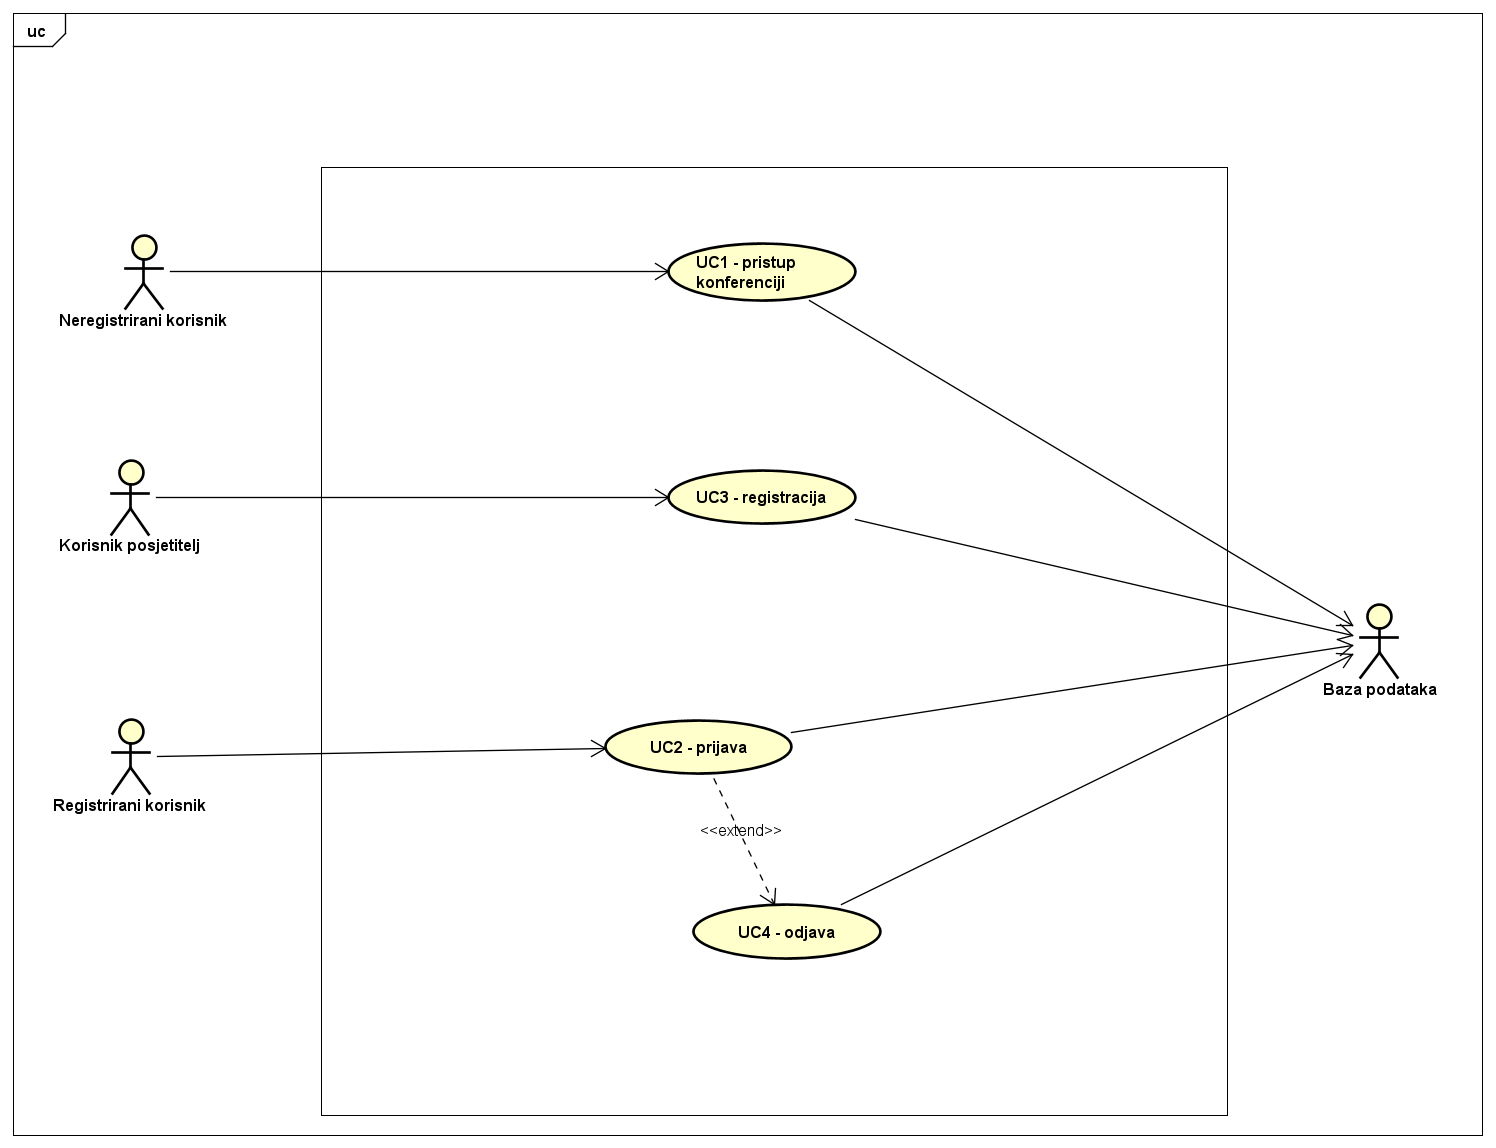
\includegraphics[width=\linewidth]{Slike/UCDiagramUserProfiles.png}
						\caption{UC dijagram za opis korisničkih računa}
					\end{figure}
					
					\begin{figure}
						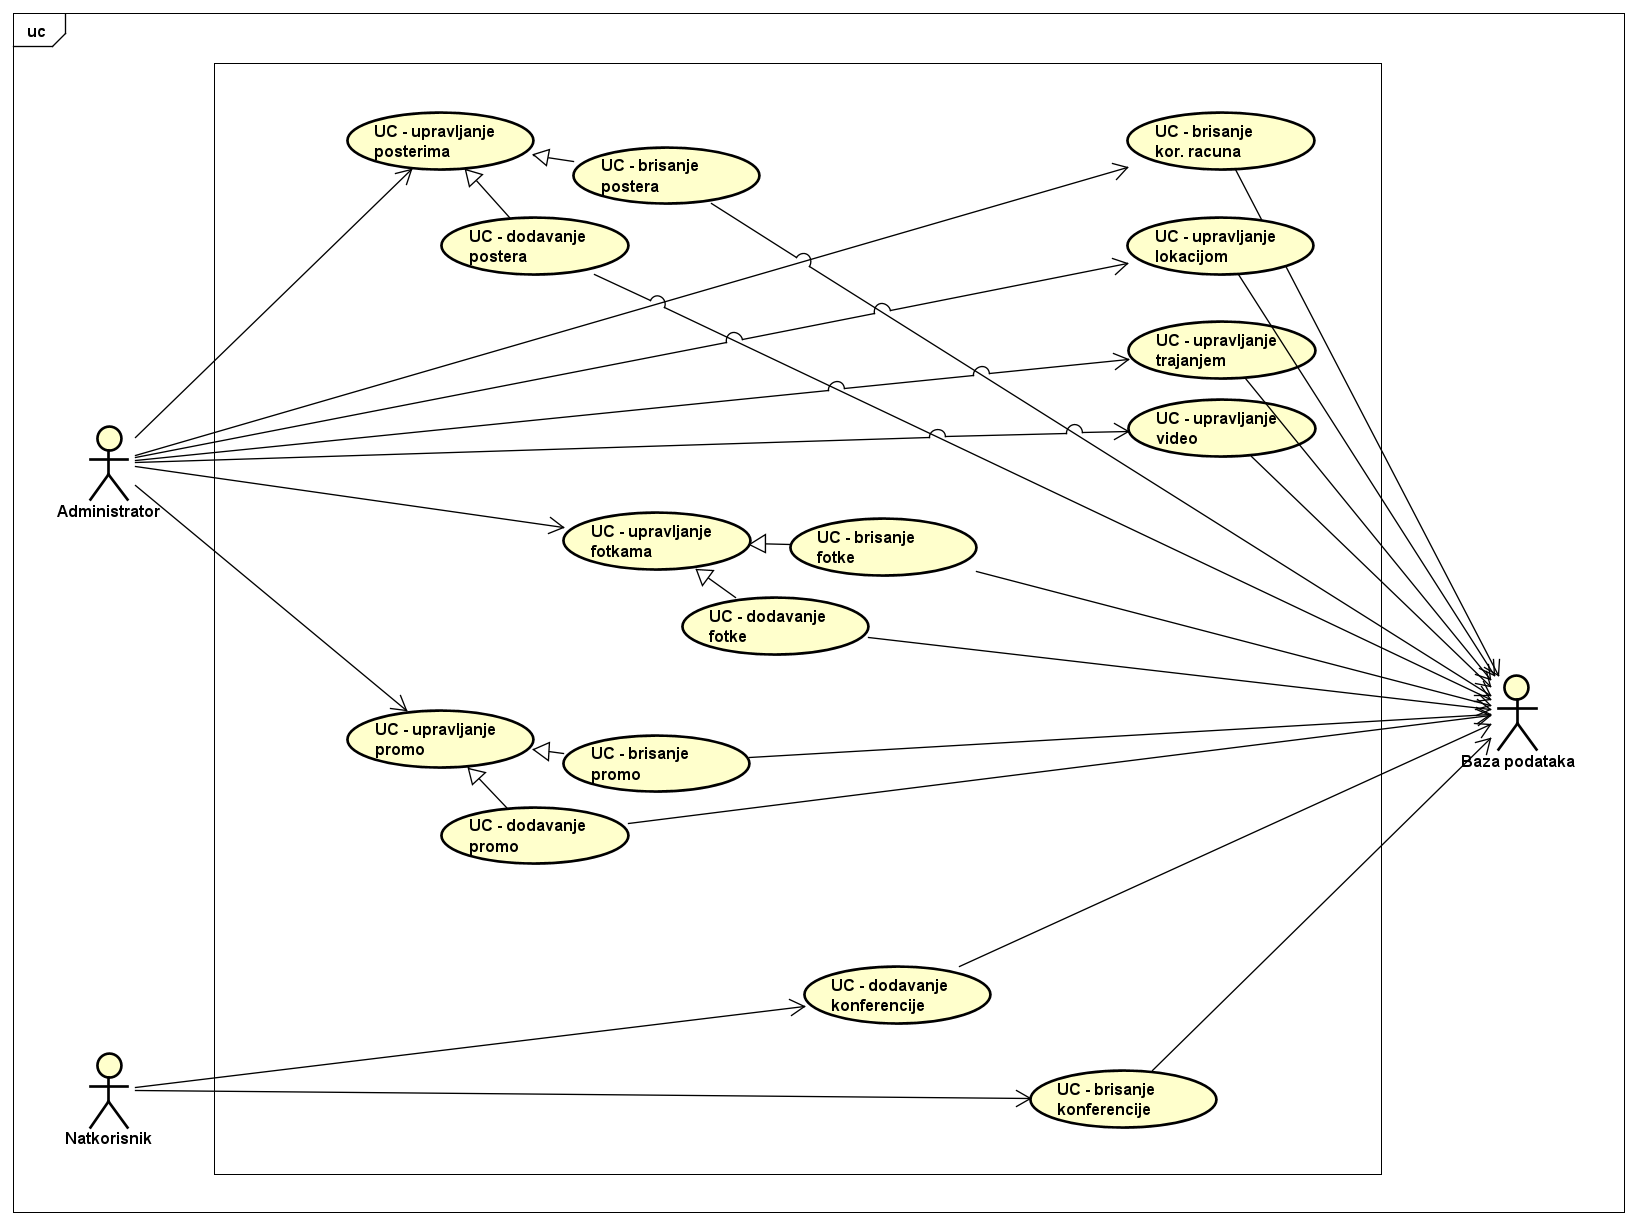
\includegraphics[width=\linewidth]{Slike/UCDiagramAdmin.png}
						\caption{UC dijagram za opis administrativnih mogućnosti}
					\end{figure}
				
					\begin{figure}
						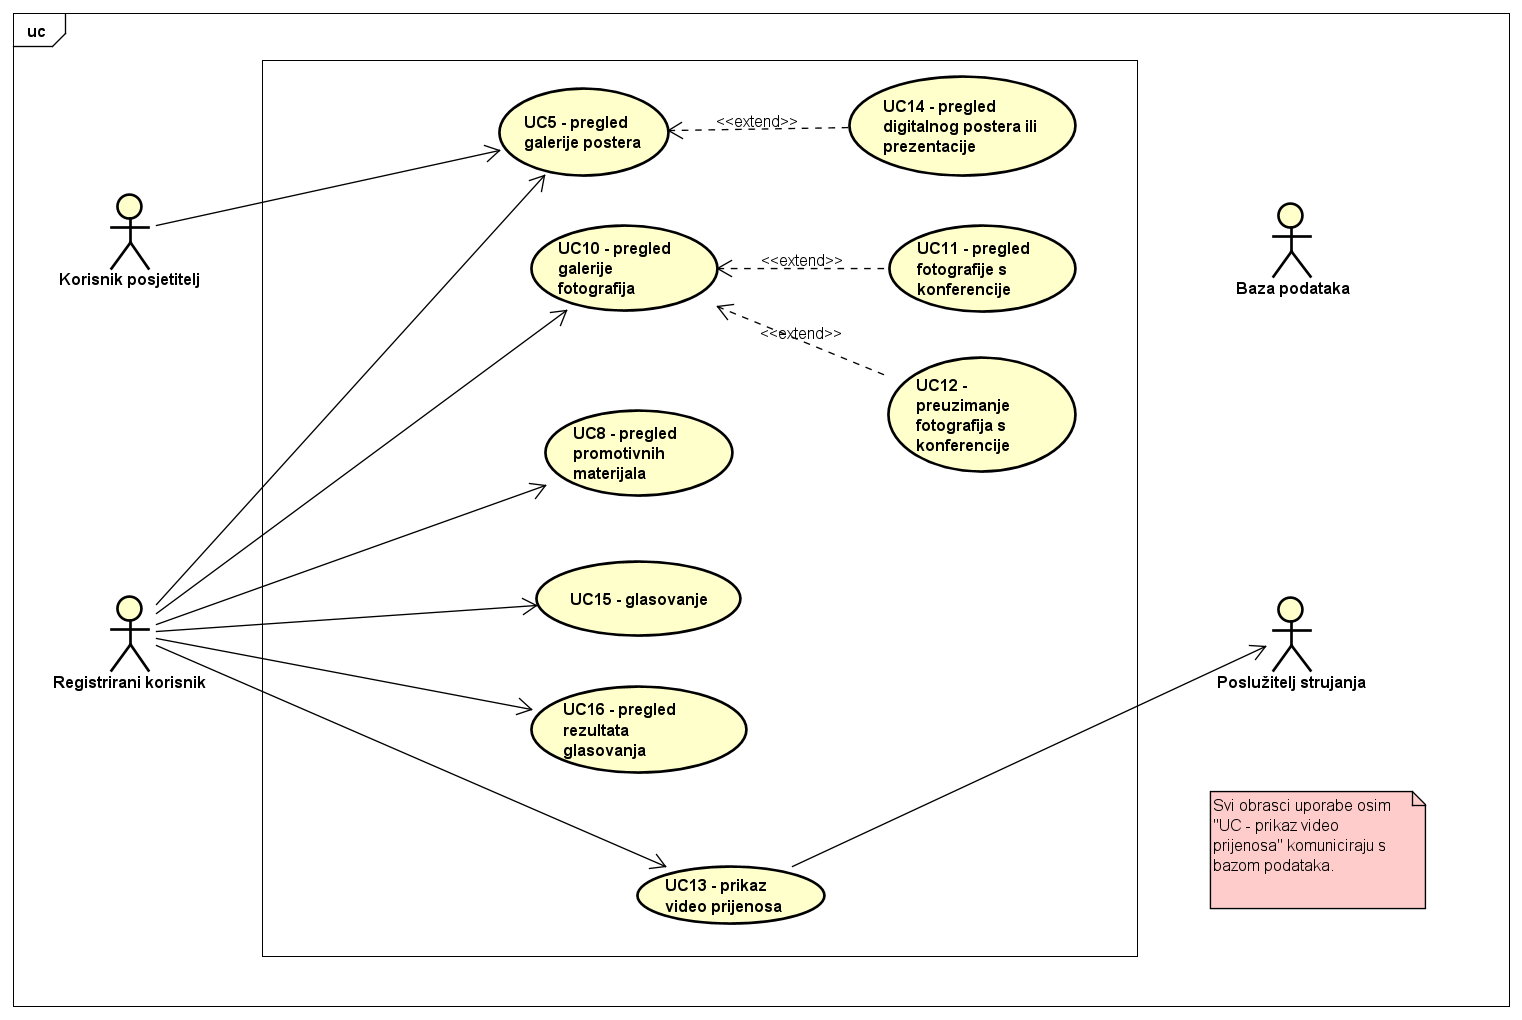
\includegraphics[width=\linewidth]{Slike/UCDiagramAppFunctionalities.png}
						\caption{UC dijagram za opis funkcionalnosti aplikacije}
					\end{figure}
				
				\eject		
			
			\clearpage
			\subsection{Sekvencijski dijagrami}
				
				\subsubsection{Obrazac uporabe UC15 - Glasovanje}
				Registrirani korisnik odabire opciju za pregled svih postera. U galeriji postera odabire jedan poster. Pojavljuje se opcija za glasovanje za odabrani poster. Klikom na tu opciju aplikacija šalje zahtjev bazi podataka kojim provjerava je li prijavljeni korisnik već glasao, te ako jest zabranjuje mu daljnje glasanje. Ukoliko korisnik nije glasao, baza podataka sprema glas. Aplikacija obavještava korisnika o uspješnom glasanju.
				
				\begin{figure}[hp!]
				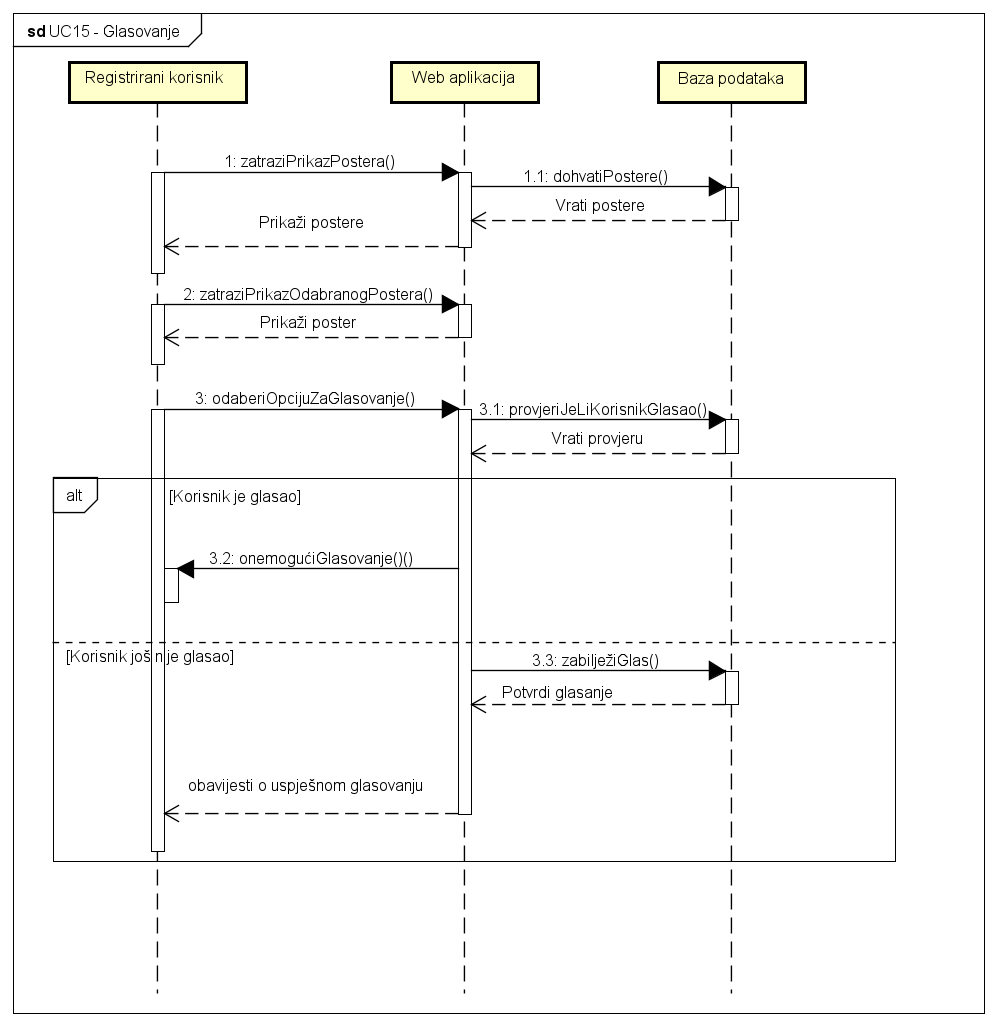
\includegraphics[width=\linewidth]{Slike/SD_Glasanje.png}
				\caption{Sekvencijski dijagram za UC15 - Glasovanje}
				\end{figure}
				
				\newpage
				
				\subsubsection{Obrazac uporabe UC18 - Upravljanje digitalnim posterima}
				Administrator odabire opciju "Galerija postera". Poslužitelj dohvaća popis postera iz baze podataka te ih prikazuje administratoru, kome se uz njih prikazuje i gumb predviđen za upravljanje digitalnim posterima. Pritiskom na njega otvara se posebno sučelje za upravljanje digitalnim posterima koje omogućava dodavanje i brisanje digitalnih postera.
				
				\subsubsection{Obrazac uporabe UC19 - Dodavanje digitalnog postera}
				Administrator pritišće gumb za dodavanje novog postera. Poslužitelj zatraži unos osnovnih podataka o posteru i  prijenos lokalne datoteke postera - administratoru se upit prikazuje kao novo otvoreni prozor. Administrator unosi podatke. Poslužitelj traži potvrdu promjena i čeka odgovor. Nakon potvrde promjena poslužitelj sprema podatke vezane uz poster u bazu podataka, a ona vraća potvrdu izmjene.
				
				\subsubsection{Obrazac uporabe UC20 - Brisanje digitalnog postera}
				Administrator odabire digitalni poster koji želi obrisati. Poslužitelj dohvaća podatke o posteru iz baze podataka. Administrator odabire opciju brisanja digitalnog postera. Poslužitelj šalje upit za potvrdu brisanja. Nakon što administrator potvrdi brisanje postera, poslužitelj ga briše iz baze podataka koja vraća potvrdu izmjene.
				
				\newpage
				
				\begin{figure}[hp!]
					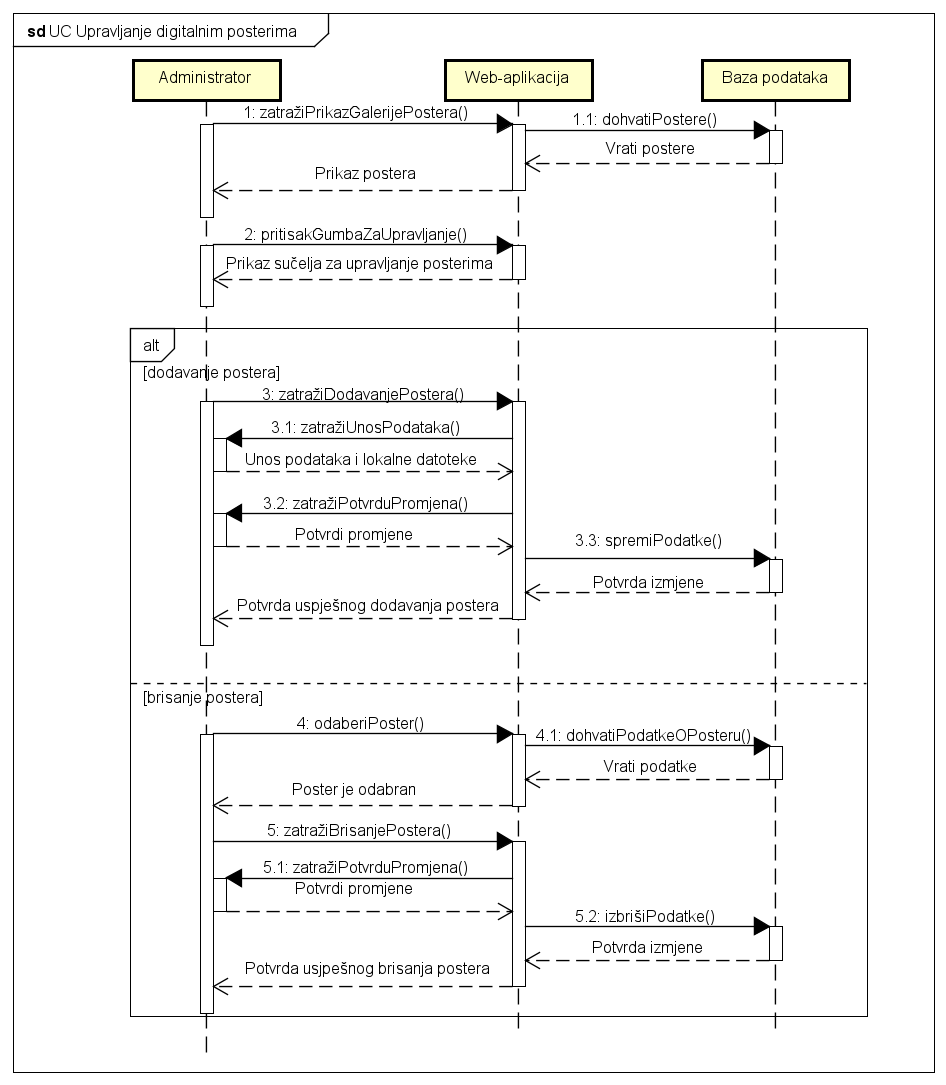
\includegraphics[width=\linewidth]{Slike/SD_UpravljanjePosterima.png}
					\caption{Sekvencijski dijagram za UC18 - Upravljanje posterima}
				\end{figure}
				
				\newpage
				
				\subsubsection{Obrazac uporabe UC31 - Slanje poruke e-pošte}
				Nakon što je glasovanje završeno šalju se tri vrste automatiziranih poruka e-pošte. Prvim trima autorima po broju glasova šalje se poziv na dodjelu nagrade. Svim autorima, bez obzira na njihov rang šalje se poruka o njihovom rangu. Svim registriranim korisnicima šalje se obavijest o mjestu i vremenu dodjele nagrade. Iste poruke se pojavljuju kao obavijesti u aplikaciji.
				
				\begin{figure}[hp!]
					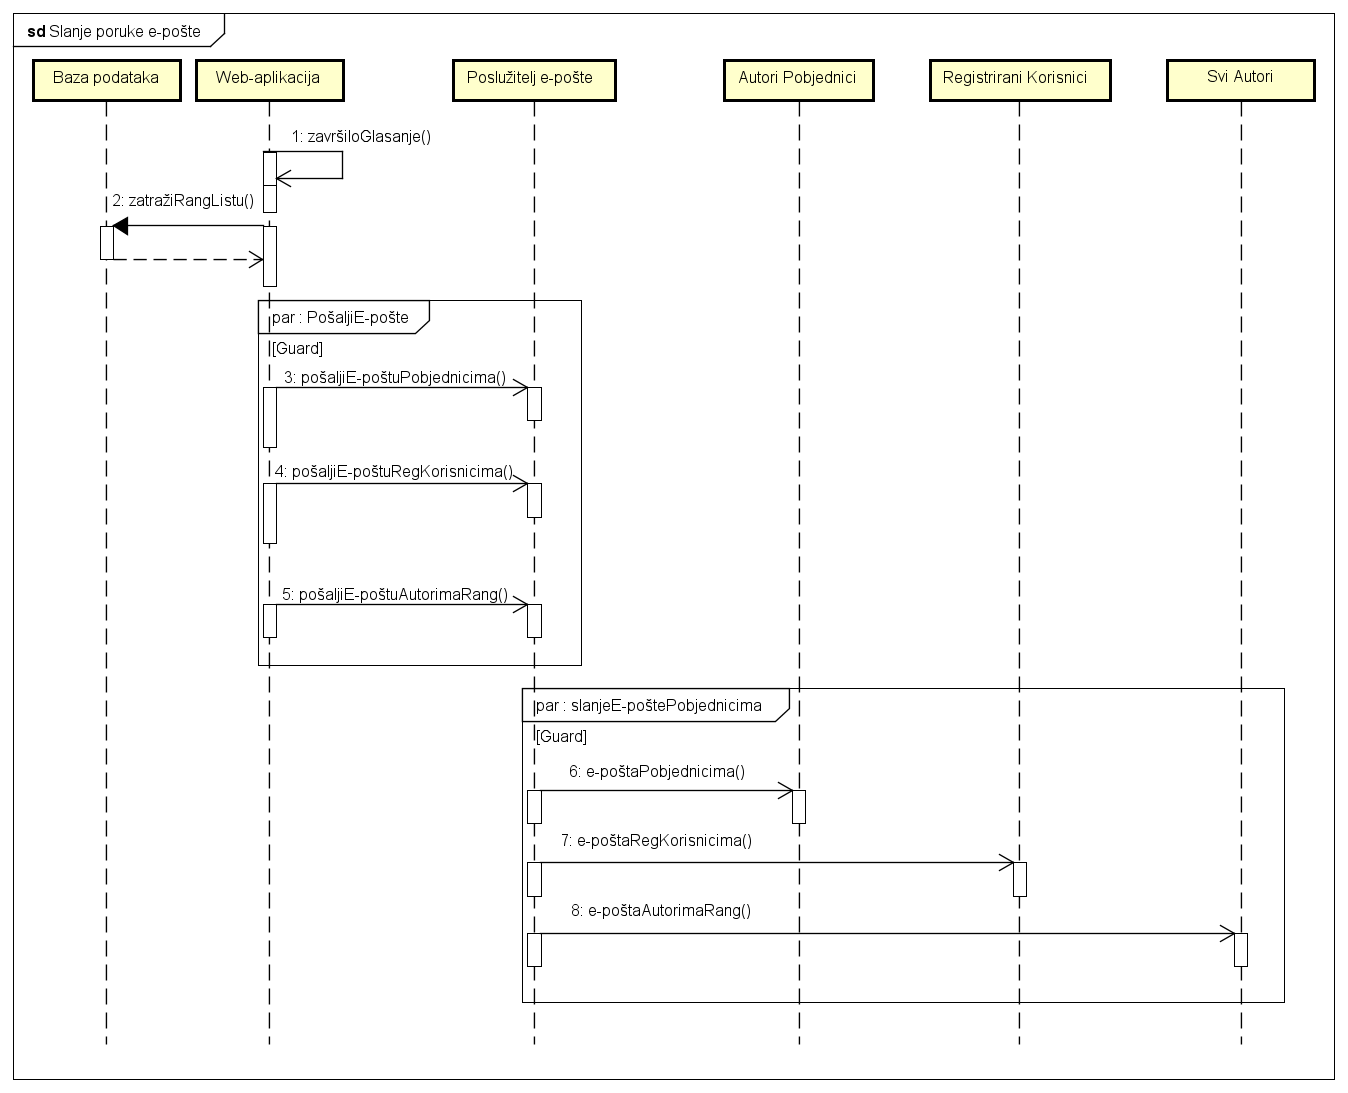
\includegraphics[width=\linewidth]{Slike/SD_SlanjeEPoste.png}
					\caption{Sekvencijski dijagram za UC31 - Slanje e-pošte}
				\end{figure}
				
				\newpage
				
				\eject
			
		\section{Ostali zahtjevi}
		
			 \begin{itemize}
			 	\item Maksimalni broj glasovanja po osobi je 1
			 	\item Glasovanje je moguće samo tijekom određenog vremenskog razdoblja koje je određeno trajanjem konferencije
			 	\item Sustav treba podržavati rad više korisnika u stvarnom vremenu.
			 	\item Korisničko sučelje i sustav moraju podržavati hrvatsku abecedu (dijakritičke
			 	znakove) pri unosu i prikazu tekstualnog sadržaja
			 	\item Izvršavanje dijela programa u kojem se pristupa bazi podataka ne smije trajati dulje od nekoliko sekundi
			 	\item Sustav treba biti implementiran kao web aplikacija koristeći objektno-orijentirane
			 	jezike
			 	\item Neispravno korištenje korisničkog sučelja ne smije narušiti funkcionalnost i rad sustava
			 	\item Sustav treba biti jednostavan za korištenje, korisnici se moraju znati koristiti sučeljem bez opširnih uputa
			 	\item Nadogradnja sustava ne smije narušavati postojeće funkcionalnosti sustava
			 	\item Veza s bazom podataka mora biti kvalitetno zaštićena, brza i otporna na vanjske greške
			 	\item Pristup sustavu mora biti omogućen iz javne mreže protokolom HTTPS
			 \end{itemize}
			 
			 
			 
	